\documentclass[tikz,border=2pt]{standalone}
\usepackage{amsmath}
\usepackage{pgfplots}
\pgfplotsset{compat=1.18}
\usetikzlibrary{arrows.meta}
\begin{document}
% Exercise 7.3: pricing the new column A_3=(1,2,1) at y^*=(0,3/2,1) gives y^{*T}A_3=0+3+1=4, so the reduced
% cost is 4-c_3: c_3=3 gives 1 (basis stays optimal), c_3=6 gives -2 (x_3 enters); threshold c_3=4.
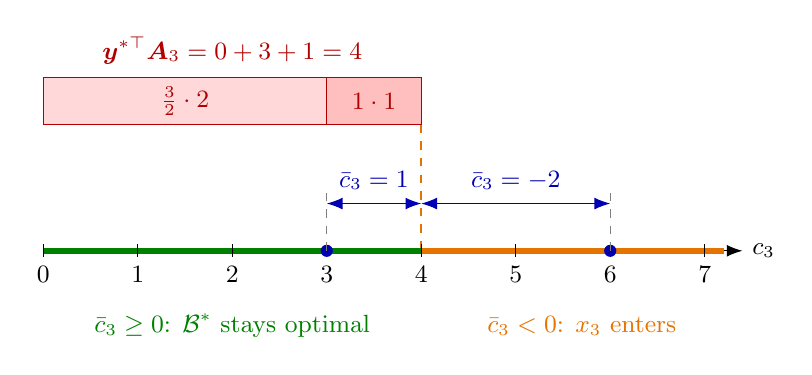
\begin{tikzpicture}[font=\small, >={Latex[length=2mm]}, x=1.2cm, y=1cm]
  % value of the resources one unit of x_3 uses
  \draw[red!70!black, fill=red!15] (0,1.6) rectangle (3,2.2);
  \draw[red!70!black, fill=red!25] (3,1.6) rectangle (4,2.2);
  \node[red!70!black] at (1.5,1.9) {$\tfrac{3}{2}\cdot2$};
  \node[red!70!black] at (3.5,1.9) {$1\cdot1$};
  \node[red!70!black, anchor=south] at (2,2.25) {$\boldsymbol{y}^{*\top}\boldsymbol{A}_3=0+3+1=4$};
  % threshold
  \draw[orange!90!black, thick, dashed] (4,1.6) -- (4,0);
  % c_3 axis
  \draw[->] (0,0) -- (7.4,0) node[right] {$c_3$};
  \draw[green!50!black, line width=2pt] (0,0) -- (4,0);
  \draw[orange!90!black, line width=2pt] (4,0) -- (7.2,0);
  \foreach \x in {0,...,7} \draw (\x,0.08) -- (\x,-0.08) node[below] {$\x$};
  % the two prices of Exercise 7.3 and their reduced costs 4-c_3
  \fill[blue!70!black] (3,0) circle (2.2pt) (6,0) circle (2.2pt);
  \draw[gray, thin, dashed] (3,0) -- (3,0.8) (6,0) -- (6,0.8);
  \draw[<->, blue!70!black] (3,0.6) -- (4,0.6);
  \draw[<->, blue!70!black] (4,0.6) -- (6,0.6);
  \node[blue!70!black, anchor=south] at (3.5,0.65) {$\bar{c}_3=1$};
  \node[blue!70!black, anchor=south] at (5,0.65) {$\bar{c}_3=-2$};
  % verdicts
  \node[green!50!black] at (2,-0.95) {$\bar{c}_3\geq0$: $\mathcal{B}^*$ stays optimal};
  \node[orange!90!black] at (5.7,-0.95) {$\bar{c}_3<0$: $x_3$ enters};
\end{tikzpicture}
\end{document}
